% Template of basic phisics experiment 基于 article template，在此基础上做修改
% 设定文章编码类型，正文字号为五号则 zihao=5，正文字号为小四则 zihao=-4
\documentclass[zihao=5, UTF8]{article}		


% 自定义宏定义
\def\N{\mathbb{N}}
\def\F{\mathbb{F}}
\def\Z{\mathbb{Z}}
\def\Q{\mathbb{Q}}
\def\R{\mathbb{R}}
\def\C{\mathbb{C}}
\def\T{\mathbb{T}}
\def\S{\mathbb{S}}
\def\A{\mathbb{A}}
\def\I{\mathscr{I}}
\def\d{\mathrm{d}}
\def\p{\partial}


% 物理实验报告所需的其它宏包
\usepackage{ulem}   % \uline 下划线支持

% 导入基本宏包
\usepackage[UTF8]{ctex}     % 设置文档为中文语言
\usepackage[colorlinks, linkcolor=blue, anchorcolor=blue, citecolor=blue, urlcolor=blue]{hyperref}  % 宏包：自动生成超链接 (此宏包与标题中的数学环境冲突)
% \usepackage{docmute}    % 宏包：子文件导入时自动去除导言区，用于主/子文件的写作方式，\include{./51单片机笔记}即可。注：启用此宏包会导致.tex文件capacity受限。
\usepackage{amsmath}    % 宏包：数学公式
\usepackage{mathrsfs}   % 宏包：提供更多数学符号
\usepackage{amssymb}    % 宏包：提供更多数学符号
\usepackage{pifont}     % 宏包：提供了特殊符号和字体
\usepackage{extarrows}  % 宏包：更多箭头符号

% 列表环境设置
\usepackage{enumitem}   % 宏包：列表环境设置
    \setlist[enumerate]{itemsep=0pt, parsep=0pt, topsep=0pt, partopsep=0pt, leftmargin=3.5em} 
    \setlist[itemize]{itemsep=0pt, parsep=0pt, topsep=0pt, partopsep=0pt, leftmargin=3.5em}
    \newlist{circledenum}{enumerate}{1} % 创建一个新的枚举环境  
    \setlist[circledenum,1]{  
        label=\protect\circled{\arabic*}, % 使用 \arabic* 来获取当前枚举计数器的值，并用 \circled 包装它  
        ref=\arabic*, % 如果需要引用列表项，这将决定引用格式（这里仍然使用数字）
        itemsep=0pt, parsep=0pt, topsep=0pt, partopsep=0pt, leftmargin=3.5em
    }  
% 文章页面 margin 设置
\usepackage[a4paper]{geometry}  % 宏包：文章页面 margin 设置
    \geometry{top=0.75in}
    \geometry{bottom=0.75in}
    \geometry{left=0.75in}
    \geometry{right=0.75in}   % 设置上下左右页边距
    \geometry{marginparwidth=1.75cm}    % 设置边注距离（注释、标记等）

% 自定义数学环境
\usepackage{amsthm} % 宏包：数学环境配置
% theorem-line 环境自定义
    \newtheoremstyle{MyLineTheoremStyle}% <name>
        {11pt}% <space above>
        {11pt}% <space below>
        {}% <body font> 使用默认正文字体
        {}% <indent amount>
        {\bfseries}% <theorem head font> 设置标题项为加粗
        {：}% <punctuation after theorem head>
        {.5em}% <space after theorem head>
        {\textbf{#1}\thmnumber{#2}\ \ (\,\textbf{#3}\,)}% 设置标题内容顺序
    \theoremstyle{MyLineTheoremStyle} % 应用自定义的定理样式
    \newtheorem{LineTheorem}{Theorem.\,}
% theorem-block 环境自定义
    \newtheoremstyle{MyBlockTheoremStyle}% <name>
        {11pt}% <space above>
        {11pt}% <space below>
        {}% <body font> 使用默认正文字体
        {}% <indent amount>
        {\bfseries}% <theorem head font> 设置标题项为加粗
        {：\\ \indent}% <punctuation after theorem head>
        {.5em}% <space after theorem head>
        {\textbf{#1}\thmnumber{#2}\ \ (\,\textbf{#3}\,)}% 设置标题内容顺序
    \theoremstyle{MyBlockTheoremStyle} % 应用自定义的定理样式
    \newtheorem{BlockTheorem}[LineTheorem]{Theorem.\,} % 使用 LineTheorem 的计数器
% definition 环境自定义
    \newtheoremstyle{MySubsubsectionStyle}% <name>
        {11pt}% <space above>
        {11pt}% <space below>
        {}% <body font> 使用默认正文字体
        {}% <indent amount>
        {\bfseries}% <theorem head font> 设置标题项为加粗
        {：\\ \indent}% <punctuation after theorem head>
        {0pt}% <space after theorem head>
        {\textbf{#3}}% 设置标题内容顺序
    \theoremstyle{MySubsubsectionStyle} % 应用自定义的定理样式
    \newtheorem{definition}{}


% 有色文本框及其设置
\usepackage[dvipsnames,svgnames]{xcolor}    %设置插入的文本框颜色
\usepackage[strict]{changepage}     % 提供一个 adjustwidth 环境
\usepackage{framed}     % 实现方框效果
    \definecolor{graybox_color}{rgb}{0.95,0.95,0.96} % 文本框颜色。修改此行中的 rgb 数值即可改变方框纹颜色，具体颜色的rgb数值可以在网站https://colordrop.io/ 中获得。（截止目前的尝试还没有成功过，感觉单位不一样）（找到喜欢的颜色，点击下方的小眼睛，找到rgb值，复制修改即可）
    \newenvironment{graybox}{%
    \def\FrameCommand{%
    \hspace{1pt}%
    {\color{gray}\small \vrule width 2pt}%
    {\color{graybox_color}\vrule width 4pt}%
    \colorbox{graybox_color}%
    }%
    \MakeFramed{\advance\hsize-\width\FrameRestore}%
    \noindent\hspace{-4.55pt}% disable indenting first paragraph
    \begin{adjustwidth}{}{7pt}%
    \vspace{2pt}\vspace{2pt}%
    }
    {%
    \vspace{2pt}\end{adjustwidth}\endMakeFramed%
    }

% 各级标题自定义设置
\usepackage{titlesec}   
    % section标题自定义设置 
    \titleformat{\section}[hang]{\normalfont\huge\bfseries\centering}{第\,\thesection\,部分}{20pt}{}
    % subsection标题自定义设置 
    \titleformat{\subsection}[hang]{\normalfont\Large\bfseries}{\,\thesubsection\,}{8pt}{}
    % subsubsection标题自定义设置
    \titleformat{\subsubsection}[hang]{\normalfont\large\bfseries}{\,\thesubsubsection\,}{6pt}{}

% 外源代码插入设置
\usepackage{matlab-prettifier}
    \lstset{
        style=Matlab-editor,  % 继承matlab代码颜色等
    }
\usepackage[most]{tcolorbox} % 引入tcolorbox包 
\usepackage{listings} % 引入listings包
    \tcbuselibrary{listings, skins, breakable}
    \lstdefinestyle{matlabstyle}{
        language=Matlab,
        basicstyle=\small,
        breakatwhitespace=false,
        breaklines=true,
        captionpos=b,
        keepspaces=true,
        numbers=left,
        numbersep=15pt,
        showspaces=false,
        showstringspaces=false,
        showtabs=false,
        tabsize=2
    }
    \newtcblisting{matlablisting}{
        arc=0pt,
        top=0pt,
        bottom=0pt,
        left=1mm,
        listing only,
        listing style=matlabstyle,
        breakable,
        colback=white   % 选一个合适的颜色
    }

% table 支持
\usepackage{booktabs}   % 宏包：三线表
\usepackage{tabularray} % 宏包：表格排版
\usepackage{longtable}  % 宏包：长表格
\usepackage{tabularx}  % 宏包：宽表格
\usepackage{multirow}  % 宏包：表格中一格显示多个项目

% figure 设置
\usepackage{graphicx}  % 支持 jpg, png, eps, pdf 图片 
\usepackage{svg}       % 支持 svg 图片
    \svgsetup{
        % 指向 inkscape.exe 的路径
        inkscapeexe = C:/aa_MySame/inkscape/bin/inkscape.exe, 
        % 一定程度上修复导入后图片文字溢出几何图形的问题
        inkscapelatex = false                 
    }


% 图表进阶设置
\usepackage{float}     % 图表位置浮动设置 
\usepackage{caption}    % 图注、表注
    \captionsetup[figure]{name=图}  
    \captionsetup[table]{name=表}
    \captionsetup{labelfont=bf, font=small}

% 文章默认字体设置
    \usepackage{fontspec}   % 宏包：字体设置
       \setmainfont{SimSun}    % 设置中文字体为宋体字体
      \setCJKmainfont[AutoFakeBold=3]{SimSun} % 设置加粗字体为 SimSun 族，AutoFakeBold 可以调整字体粗细^     \setmainfont{Times New Roman} % 设置英文字体为Times New Roman


% 其它设置
    % equation 公式编号设置
        \makeatletter  
        \renewcommand{\theequation}{\thesection.\arabic{equation}}  
        \makeatother
    % 脚注设置
        \renewcommand\thefootnote{\ding{\numexpr171+\value{footnote}}}
    % 参考文献引用设置
        \bibliographystyle{unsrt}   % 设置参考文献引用格式为unsrt
        \newcommand{\upcite}[1]{\textsuperscript{\cite{#1}}}     % 自定义上角标式引用
    % 文章序言设置
        \newcommand{\cnabstractname}{序言}
        \newenvironment{cnabstract}{%
            \par\Large
            \noindent\mbox{}\hfill{\bfseries \cnabstractname}\hfill\mbox{}\par
            \vskip 2.5ex
            }{\par\vskip 2.5ex}


% 页眉页脚设置
\usepackage{fancyhdr}   %宏包：页眉页脚设置
    \pagestyle{fancy}
    \fancyhf{}
    \cfoot{\thepage}
    \renewcommand\headrulewidth{1pt}
    \renewcommand\footrulewidth{0pt}
    \rhead{\bfseries 分组序号: YK04-2}    
    \chead{《基础物理实验》实验报告,\ 韩初晓,\ 2023K8009908002}
    \lhead{2024.10.10}

% 文档信息设置
%\title{这里是标题\\The Title of the Report}
%\author{丁毅\\ \footnotesize 中国科学院大学，北京 100049\\ Yi Ding \\ %\footnotesize University of Chinese Academy of Sciences, Beijing %100049, China}
%\date{\footnotesize 2024.8 -- 2025.1}

% 开始编辑文章

\begin{document}
\noindent\begin{flushright}
    \zihao{2}{分组序号: YK04-2}
\end{flushright}

\setCJKfamilyfont{boldsong}[AutoFakeBold = {2.17}]{SimSun}
\newcommand*{\boldsong}{\CJKfamily{boldsong}}


\begin{center}\large
    \noindent{\Huge\bfseries\boldsong《基础物理实验》实验报告 }
    \\\vspace{0.4cm}
    \noindent\textit{
        \textbf{\boldsong 实验名称：}\uline{\hspace{1.7cm} 测量金属的杨氏模量\hspace{1.7cm}}\hspace{0.4cm} 
        指导教师：\uline{\hspace{1.0cm}董政\hspace{1.0cm}}}
    \\\vspace{0.1cm}
    \noindent\textit{
        姓名：\uline{\,\,\,韩初晓\,\,\,}\hspace{0.2cm}
        学号：\uline{\,\,\,{\upshape 2023K8009908002}\,\,\,}\hspace{0.2cm}
        专业：\uline{\,\,\,计算机科学与技术\,\,\,}\hspace{0.2cm}
        班级：\uline{\,\,\,\upshape{2306}\,\,\,}}
    \\\vspace{0.1cm}
    \noindent\textit{
        实验日期：\uline{\,\,{\upshape 2024.11.7}\,\,}\hspace{0.2cm}
        实验地点：\uline{\,\,\,教学楼{\upshape710}\,\,\,}\hspace{0.2cm}
        是否调课/补课：\uline{\hspace{0.5cm}否\hspace{0.5cm}}\hspace{0.2cm}
        成绩：\uline{\hspace{2cm}}}
\end{center}
% \vspace{-0.2cm}
\noindent\rule{\textwidth}{0.1em}   % 分割线

% 控制目录不换页
\vspace{1cm}
\setcounter{tocdepth}{2}  % 目录深度为 2（不显示 subsubsection）
\noindent\begin{minipage}{\textwidth}\centering
\tableofcontents\thispagestyle{fancy}   % 显示页码、页眉等   
\end{minipage}  
\newpage

\section{实验目的}
\begin{enumerate}
    \item 了解静态、动态和霍尔法测量杨氏模量。
    \item 学习使用霍尔传感器、读数显微镜、显微镜等实验设备。
    \item 学习误差分析方法，如图示法和最小二乘法处理实验数据。
    \item 学习使用外延法处理实验数据。
    \item 了解换能器的功能，熟悉测试仪器及示波器的使用。
\end{enumerate}

\section{拉伸法测量杨氏模量}\thispagestyle{fancy} 

\subsection{实验用具}

\begin{table}[h!]
\centering
\caption{实验用具及主要参数}
\begin{tabular}{|c|c|c|}
\hline
实验用具 & 型号/规格 & 主要参数 \\ \hline
CCD 杨氏弹性模量测量仪 & LB-YM1 型 & \begin{tabular}[c]{@{}c@{}}不锈钢双柱，高约 85cm \\ 金属丝（钼丝或钢丝）长 60cm，可调节 \\ 彩色液晶监视器 \\ 分化板刻度范围 4mm，分度值 0.05mm \\ CCD 系统放大倍率 60 倍，分辨率 480TVL \\ 砝码组 200g×8 + 100g×2 \\ 测量不确定度 <5\%\end{tabular} \\ \hline
CCD 杨氏弹性模量测量仪 & YMC-2 型 & \begin{tabular}[c]{@{}c@{}}读数显微镜放大倍数 15× \\ 测量架范围 0-4mm \\ 钼丝 L=1000mm, Φ0.18mm \\ 不锈钢丝 L=1000mm, Φ0.30mm \\ 光学平台尺寸 405mm×308mm×39mm \\ 镀铬钢制砝码 250g×8\end{tabular} \\ \hline
\end{tabular}
\end{table}


\subsection{实验原理}

柱状物体受外力作用时发生形变。在弹性范围内，正应力与线应变成正比：

\[
\frac{F}{S} = Y \frac{\Delta L}{L}
\]

其中比例系数 $Y$ 是杨氏弹性模量，单位为 $N/m^2$ 或 达因/cm²，反映材料抵抗变形的能力。

拉伸法通过悬挂金属丝并加载砝码来测量杨氏模量。通过金属丝长度 $L$、直径 $d$ 和所加砝码质量 $M$ 计算力 $F=Mg$ 和横截面积 $S=\pi d^2/4$，从而得到杨氏模量：

\[ Y = \frac{4FL}{\pi d^2 \Delta L} \]

由于金属丝伸长量极小（约 $10^{-1}$ mm），使用显微镜和 CCD 成像系统测量。金属丝末端连接十字叉丝板和砝码盘，增加砝码使金属丝受力增大，导致叉丝板位移 $\Delta L$。通过显微镜观察叉丝板的移动，结合 CCD 技术记录数据实现精确测量。


\subsection{实验内容}

\subsubsection*{仪器调节}

\begin{enumerate}
    \item 调节支架确保金属丝竖直，检查两支柱是否垂直，必要时调整支撑脚。
    \item 加载一个250g砝码以拉直金属丝，检查是否存在弯曲情况，若有需更换金属丝。
    \item 调节CCD摄像机使其对准叉丝组分划板。
    \item 微调CCD摄像机位置直至屏幕显示清晰影像，确保分划板刻度位于屏幕中央。
\end{enumerate}

\subsubsection*{测量步骤}

1. 先放砝码拉直金属丝，确认分划板稳固，避免旋转。
   - 注意分划板刻度不应高于3mm。
   
2. 记录无砝码时的初始读数$l_0=0$，每次添加200g砝码，记录相应读数$l_i$($i=1,2,...,8$)。
   - 减少砝码时重复上述过程，记录$l'_i$。
   - 动作轻柔以防砝码盘震动影响读数。

3. 对同一负荷下的读数取平均值$\bar{l}_i$，利用逐差法计算荷重增减四个砝码时的平均偏移量$\Delta L$。

4. 使用钢卷尺测量上下夹头间金属丝的总长度$L$。

5. 使用螺旋测微器测量金属丝直径$d$，考虑不同部位的差异性。

6. 根据公式计算杨氏模量$Y$：
   \[
   Y = \frac{4MgL}{\pi d^2 \Delta L}
   \]
   其中，$\Delta L$与砝码数量$M$相关，代表单个或多个砝码引起的变化。

\subsection{数据整理和计算}

\subsubsection{钼丝长度测量}
钼丝长度: $L = 788.1$mm 仪器误差 $e = 2.0$mm, 最小分度值 $1$mm

\[ u(L) = \sqrt{u_{B1}(L)^2 + u_{B2}(L)^2} = \sqrt{1^2 + \left(\frac{2}{\sqrt{3}}\right)^2} = 1.52 mm \]

记作 $1.5$mm $\bar{L} = 788.1 \pm 1.5 $，其相对不确定度为

\[ \frac{u(L)}{\bar{L}} = \frac{1.5}{788.1} \times 100 \% = 0.19 \% \]

\subsubsection{钼丝直径测量}

\begin{table}[htb]
    \centering
    \begin{tabular}{|c|c|c|c|c|c|c|c|}
        \hline
        测量次数 & 1 & 2 & 3 & 4 & 5 & 6 & 平均值 \\
        \hline
        d/mm & 0.190 & 0.191 & 0.189 & 0.185 & 0.185 & 0.188 & 0.188 \\
        \hline
    \end{tabular}
\end{table}

铜丝直径平均值 $0.188$mm, 允差 $0.004$mm

\[ u_A(d) = \sqrt{\frac{\sum_{i=1}^{n}(d_i-\bar{d})^2}{n(n-1)}} = 1.032 \times 10^{-3} mm \]

\[ u_B(d) = \frac{\epsilon}{\sqrt{3}} = 2.3094 \times 10^{-3} mm \]

\[ u(d) = \sqrt{u_A(d)^2 + u_B(d)^2} = 2.5295 \times 10^{-3} mm \]

记 $u(d)$ 为 $3 \times 10^{-3}$mm，其相对不确定度为

\[ \frac{u(d)}{\bar{d}} = \frac{3 \times 10^{-3}}{0.188} \times 100 \% = 1.6 \% \]

于是钼丝直径为

\[ \bar{d} = 0.188 \pm 0.003 mm \]

\subsubsection{钼丝长度变化测量}

初始示数$l_0 = 0.01$mm，千分尺误差$e = 0.005$mm。

\begin{table}[H]
  \centering
	\begin{tabular}{|l|l|llc|lll|}
		\hline
		\multicolumn{1}{|c|}{\multirow{2}{*}{序号i}} & \multicolumn{1}{c|}{\multirow{2}{*}{\begin{tabular}[c]{@{}c@{}}砝码质量\\ M/g\end{tabular}}} & \multicolumn{3}{c|}{叉丝读数}                                                                                                                                                                                                    & \multicolumn{1}{c|}{\multirow{2}{*}{\begin{tabular}[c]{@{}c@{}}liMi\\ /mm·g\end{tabular}}} & \multicolumn{1}{c|}{\multirow{2}{*}{\begin{tabular}[c]{@{}c@{}}示数差值\\ $\Delta \bar{l_i}=\bar{l_{i+4}}-\bar{l_i}$\end{tabular}}} & \multicolumn{1}{c|}{\multirow{2}{*}{\begin{tabular}[c]{@{}c@{}}不确定度\\ $\Delta \bar{l_i}$\end{tabular}}} \\ \cline{3-5}
		\multicolumn{1}{|c|}{}                     & \multicolumn{1}{c|}{}                                                                    & \multicolumn{1}{c|}{\begin{tabular}[c]{@{}c@{}}加载$l_i$\\ /mm\end{tabular}} & \multicolumn{1}{c|}{\begin{tabular}[c]{@{}c@{}}卸载$l_i$\\ /mm\end{tabular}} & \multicolumn{1}{c|}{\begin{tabular}[c]{@{}c@{}}平均值$\bar{l_i}$\\ /mm\end{tabular}} & \multicolumn{1}{c|}{}                                                                      & \multicolumn{1}{c|}{}                                                                         & \multicolumn{1}{c|}{}                                                                   \\ \hline
		1                                          & 250                                                                                      & \multicolumn{1}{c|}{0.25}                                               & \multicolumn{1}{c|}{0.32}                                               & 0.285                                                                     & \multicolumn{1}{c|}{71.25}                                                                   & \multicolumn{1}{c|}{0.96}                                                                     & \multirow{7}{*}{0.003}                                                               \\ \cline{1-7}
		2                                          & 500                                                                                      & \multicolumn{1}{c|}{0.51}                                               & \multicolumn{1}{c|}{0.55}                                               & 0.53                                                                     & \multicolumn{1}{c|}{265}                                                                   & \multicolumn{1}{c|}{0.94}                                                                     &                                                                                         \\ \cline{1-7}
		3                                          & 750                                                                                      & \multicolumn{1}{c|}{0.76}                                               & \multicolumn{1}{c|}{0.77}                                               & 0.765                                                                    & \multicolumn{1}{c|}{573.75}                                                                   & \multicolumn{1}{c|}{0.93}                                                                     &                                                                                         \\ \cline{1-7}
		4                                          & 1000                                                                                      & \multicolumn{1}{c|}{1.00}                                               & \multicolumn{1}{c|}{1.02}                                               & 1.01                                                                    & \multicolumn{1}{c|}{1010}                                                                   & \multicolumn{1}{c|}{0.94}                                                                     &                                                                                         \\ \cline{1-7}
		5                                          & 1250                                                                                     & \multicolumn{1}{c|}{1.23}                                               & \multicolumn{1}{c|}{1.25}                                               & 1.24                                                                     & \multicolumn{1}{c|}{1550}                                                                   & \multicolumn{1}{c|}{\multirow{4}{*}{}}                                                        &                                                                                         \\ \cline{1-6}
		6                                          & 1500                                                                                     & \multicolumn{1}{c|}{1.46}                                               & \multicolumn{1}{c|}{1.47}                                               & 1.465                                                                    & \multicolumn{1}{c|}{2197.5}                                                                    & \multicolumn{1}{c|}{}                                                                         &                                                                                         \\ \cline{1-6}
    7                                          & 1750                                                                                     & \multicolumn{1}{c|}{1.69}                                              & \multicolumn{1}{c|}{1.70}                                              & 1.695                                                                    & \multicolumn{1}{c|}{2957.5}                                                                  & \multicolumn{1}{c|}{}                                                                         &                                                                                         \\ \cline{1-6}
		8                                          & 2000                                                                                     & \multicolumn{1}{c|}{1.95}                                              & \multicolumn{1}{c|}{1.95}                                              & 1.95                                                                    & \multicolumn{1}{c|}{3900}                                                                  & \multicolumn{1}{c|}{}                                                                         &                                                                                         \\ \hline
		M                                          & 1125                                                                                      & \multicolumn{1}{c|}{\multirow{2}{*}{}}                                  & \multicolumn{1}{c|}{$\bar{\bar{l}}$}                                                  & 1.118                                                              & \multicolumn{3}{c|}{\multirow{2}{*}{}}                                                                                                                                                                                                                                               \\ \cline{1-2} \cline{4-5}
		$\sum M$                                         & 9000                                                                                     & \multicolumn{1}{c|}{}                                                   & \multicolumn{1}{c|}{$\sum \bar{l}$}                                                 & 8.94                                                                    & \multicolumn{3}{c|}{}                                                                                                                                                                                                                                                                \\ \hline
	\end{tabular}
\end{table}

\[ \bar{\Delta l} = 0.94 \, \text{mm} \]

\[ u_A(\Delta l) = \sqrt{\frac{\sum_{i=1}^{n} (l_i - \overline{l})^2}{n(n-1)}} = 0.006 \, \text{mm} \]

\[ u_{B2}(\Delta l) = \frac{e}{\sqrt{3}} = 0.002 \, \text{mm} \]

\[ u(\Delta l) = \sqrt{u_A(\Delta l)^2 + u_B(\Delta l)^2} = 0.006 \, \text{mm} \]

记 $u(\Delta l)$ 为 $1 \times 10^{-2} \, \text{mm}$，其相对不确定度为

\[ \frac{u(\Delta l)}{\bar{\Delta l}} = \frac{1 \times 10^{-2}}{0.94} \times 100 \% = 1.1 \% \]

于是钼丝的长度变化为：

\[ \Delta L = (0.94 \pm 0.01) \, \text{mm} \]

\subsubsection{用逐差法计算杨氏模量}

根据公式$Y = \frac{4\Delta MgL}{\pi d^2 \Delta L}$，杨氏模量的计算结果如下

\[Y = \frac{4 \times (1000 \times 10^{-3}) \times 9.81 \times (788.1 \times 10^{-3})}{\pi \times (0.188 \times 10^{-3})^{2} \times (0.94 \times 10^{-3})} = 2.96 \times 10^{11} \, \text{N} \cdot \text{m}^{-2} \]

我们将测量过程中得到的结果带入不确定度传递公式
\[
  \frac{u(Y)}{Y} = \sqrt{\left(\frac{u(L)}{L}\right)^2 + \left(\frac{u((\Delta l) ̅}{(\Delta l) ̅}\right)^2 + \left(2 \frac{u(d)}{d}\right)^2} = \sqrt{0.0019^2 + 0.011^2 + (2 \times 0.016)^2 } = 0.034
\]
从中解出杨氏模量的不确定度$u(Y)$

\[ u(Y) = 0.034 \times 2.96 \times 10^{11} = 0.1 \times 10^{11} \, \text{N} \cdot \text{m}^{-2} \]

由此知道

\[ Y = (2.96 \pm 0.1) \times 10^{11} \, \text{N} \cdot \text{m}^{-2} \]

以上结果，的计算相对误差为

\[
E_r (Y) = \frac{|Y - Y_0|}{Y_0} \times 100\% = \frac{(2.96 - 2.3)}{2.3} \times 100\% = 28.7\%.
\]
\subsubsection{用最小二乘法计算杨氏模量}

以质量$M$为横坐标，$\bar l_i$为纵坐标，作线性拟合，得到斜率$k$，则杨氏模量$Y = 4gL/\pi d^2 k$。

由最小二乘法的规则，我们知道$k$的表达式为

\[ 
k = \frac{\sum_{i=1}^{n} M_i \bar{l_i} - \frac{1}{n} \sum_{i=1}^{n} M_i \sum_{i=1}^{n} \bar{l_i}}{\sum_{i=1}^{n} M_i^2 - \frac{1}{n} (\sum_{i=1}^{n} M_i)^2} = \frac{12525 - \frac{9000 \times 8.94}{8}}{1.275 \times 10^7 - 1.0125 \times 10^7} = 9.4 \times 10^{-4} \, \text{mm} \cdot \text{g}^{-1}
\]
带入公式$Y = 4gL/\pi d^2 k$，得到杨氏模量

\[ Y = \frac{4 \times 9.81 \times 788.1 \times 10^{-3}}{\pi \times (0.188 \times 10^{-3})^2 \times 9.4 \times 10^{-4}} = 2.96 \times 10^{11} \, \text{N} \cdot \text{m}^{-2} \]

这一结果的相对误差是

\[ E_r (Y) = \frac{|Y - Y_0|}{Y_0} \times 100\% = \frac{(2.96 - 2.3)}{2.3} \times 100\% = 28.7\% \]

\subsubsection{用作图法计算杨氏模量}
我们以$m$为横坐标，$l_i$为纵坐标作图，画一条直线，使得点尽量在直线两侧均匀分布，在直线上找两点，得到斜率$k$，同样有$Y = 4gL/\pi d^2 k$。

\begin{figure}[H]
    \centering
    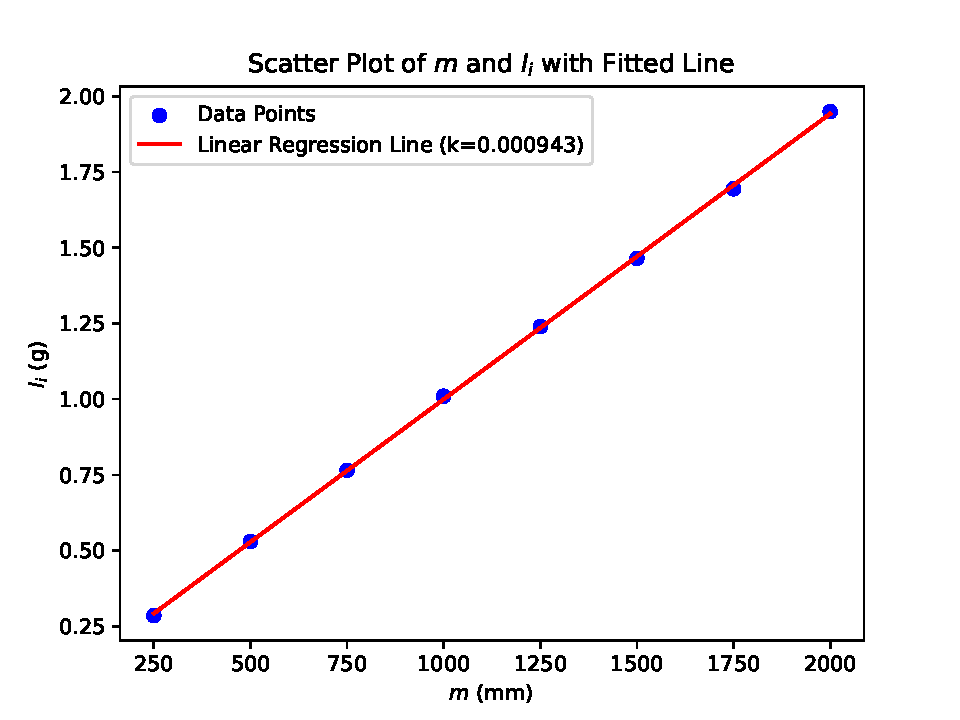
\includegraphics[width=0.6\textwidth]{./linear_regression_of_m_and_li.pdf}  % 将 "example-image" 替换为图片的文件名
\end{figure}

在图表中，拟合直线的斜率为$k = 9.43 \times 10^{-4}$mm·g$^{-1}$，带入公式$Y = 4gL/\pi d^2 k$，得到杨氏模量$Y = 2.95 \times 10^{11}$N·m$^{-2}$。

这一结果的相对误差是

\[ E_r (Y) = \frac{|Y - Y_0|}{Y_0} \times 100\% = \frac{(2.95 - 2.3)}{2.3} \times 100\% = 28.3\% \]

\subsection{总结与思考}

\subsubsection{实验过程中的问题}
在实验中我遇到了一些问题，例如在调整CCD摄像机时遇到了困难。需要将摄像机对焦并使其对准叉丝分划板，这需要一定的技巧与耐心，此外，部分CCD摄像机信号不佳，可能会出现中断蓝屏的情况。此外，测量金属丝的长度时需要测量两个螺丝之间的距离，但由于卷尺容易弯曲，并且再观察刻度时光线不甚充足，容易产生测量上的困难。此外，在增减砝码时很难做到轻拿轻放，经常在增减砝码后示数出现了较长时间的抖动，导致读数困难。此外，由于实验器材反复被同学们使用，部分同学的不当操作可能会对钼丝的性质产生影响，使得测量的结果相比于基准值有较大的偏差。

\subsubsection{进一步的思考}
为了解决实验过程中遇到的问题，我认为可以对实验器材进行一定程度的改进，例如可以在CCD摄像机上增加自动对焦按钮，以及可更换信号线的设计。此外，可以给实验台和钼丝增添方便的可拆卸设计，这样可以将钼丝拆下后在测量其长度，得到的数据将比直接使用卷尺测量的结果更加精确。此外，也可以在增加砝码的设计上进行改进，例如可以像霍尔法测量杨氏模量实验中那样，用一个旋臂来控制拉力的增减，这样可以减少示数的抖动，提高测量的准确性。

\subsubsection{思考题}

\subsubsection{思考题}

\begin{enumerate}
    \item 杨氏模量测量数据 $N$ 若不用逐差法而用作图法，如何处理？
    \begin{itemize}
      \item 使用作图法，将质量 $m_i$ 作为横坐标，$l_i$ 作为纵坐标，作出散点图，然后通过拟合直线的斜率 $k$ 计算杨氏模量 $Y$。在其中，用到了公式\[k = 4gL/\pi d^2 k\]其中 $k$ 为拟合直线的斜率。于是，杨氏模量 \[Y = 4gL/\pi d^2 k\]
    \end{itemize}
    
    \item 两根材料相同但粗细不同的金属丝，它们的杨氏模量相同吗？为什么？
    \begin{itemize}
        \item 杨氏模量是材料的内在性质，与材料的种类有关，而与其形状、尺寸无关。因此，材料相同但粗细不同的两根金属丝，其杨氏模量是相同的。
    \end{itemize}
    
    \item 本实验使用了哪些测量长度的量具？选择它们的依据是什么？它们的仪器误差各是多少？
    \begin{itemize}
        \item 本实验使用了螺旋测微器测量金属丝的直径，卷尺测量金属丝的长度，CCD摄像机测量金属丝的伸长量。
        \item 选择依据：螺旋测微器适用于测量小尺寸的精密零件厚度，钼丝的直径很小，使用螺旋测微器测量能够减小误差；卷尺适合测量较长的尺寸，因此在本实验中适合测量钼丝的长度，而CCD摄像机适合测量微小的长度变化，虽然精度不及螺旋测微器，但可以满足本实验的要求。并且在本实验中，无法使用螺旋测微器进行金属丝伸长量的测量。
        \item 查询仪器参数可知，三者的允差分别为：螺旋测微器 $0.004$mm，卷尺 $0.8$mm，CCD摄像机 $0.005$mm。
    \end{itemize}
    
    \item 在 CCD 法测定金属丝杨氏模量实验中，为什么起始时要加一定数量的底码？
    \begin{itemize}
        \item 加底码可以消除金属丝的初始松弛，使其处于适度的拉伸状态，确保在加砝码时变形更加均匀，从而获得更准确的测量结果。
    \end{itemize}
    
    \item 加砝码后标示横线在屏幕上可能上下颤动不停，不能够完全稳定时，如何判定正确读数？
    \begin{itemize}
        \item 可通过观察标示横线在上下振动过程中的平均位置，尽可能在振动幅度最小的位置进行读数，以减小读数误差。也可以用手稳定住砝码盘后再进行读数。
    \end{itemize}
    
    \item 金属丝存在折弯会使测量结果如何变化？
    \begin{itemize}
        \item 金属丝的折弯会导致一开始金属丝长度$L$的测量偏小，由此导致杨氏模量的测量结果偏小。
    \end{itemize}
    
    \item 用螺旋测微器或游标卡尺测量时，如果初始状态都不在零位，因此需要读出值减去初值，对测量值的误差有何影响？
    \begin{itemize}
        \item 若初始状态不在零位，则每次读数都需减去初始值，这可能引入固定的系统误差，因为两次测量会增加结果的不确定度。因此，测量时应尽量校准零位，确保初始读数为零，以避免误差累积。
    \end{itemize}
\end{enumerate}


\section{霍尔法测量杨氏模量}

\subsection{实验用具}

\begin{table}[H]
\centering
\caption{DHY-A 型霍尔位置传感器法杨氏模量测定仪主要参数}
\begin{tabular}{|c|c|c|}
\hline
组件 & 型号/规格 & 主要参数 \\ \hline
霍尔位置传感器法杨氏模量测定仪 & DHY-A 型 & \begin{tabular}[c]{@{}c@{}}底座固定箱 \\ SS495A 型集成霍尔位置传感器 \\ 包含测试仪、磁体、支架、加力机构\end{tabular} \\ \hline
样品 & - & 黄铜条、铸铁条 \\ \hline
磁体 & 磁铁对 & 可调节位置 \\ \hline
杠杆 & 铜材质 & 顶端装有 SS495A 型霍尔传感器 \\ \hline
读数显微镜 & - & 带有上下调节机构 \\ \hline
电子称传感器 & - & 用于加力测量 \\ \hline
平台 & - & 含水平调节机脚 \\ \hline
其他关键部件 & - & \begin{tabular}[c]{@{}c@{}}磁体调节机构、杠杆支架、铜刀口 \\ 拉力绳、水平泡、基线、立柱、加力调节旋钮\end{tabular} \\ \hline
\end{tabular}
\end{table}

\noindent
\begin{table}[h!]
\centering
\caption{实验装置及测试仪面板}
\begin{tabular}{|c|c|}
\hline
\textbf{设备名称} & \textbf{重要参数} \\ \hline
读数显微镜 & JC-10型 \\ 
& 目镜放大率：10倍 \\ 
& 物镜放大率：2倍 \\ 
& 分辨率：0.01mm \\ 
& 测量范围：0$\sim$6mm \\ \hline

电子秤传感器 & 量程：0$\sim$199.9g \\ 
& 分辨率：0.1g \\ \hline

霍尔电压表 & 量程1：0$\sim$199.9mV，分辨率0.1mV \\ 
& 量程2：0$\sim$1.999V，分辨率1mV \\ \hline

霍尔位置传感器 & 灵敏度大于250mV/mm \\ 
& 线性范围：0$\sim$2mm \\ \hline
\end{tabular}
\end{table}


\subsection{实验原理}

当霍尔元件位于磁感应强度为 \(B\) 的磁场中，并通过电流 \(I\)，则会在与磁场和电流垂直的方向上产生霍尔电势差 \(U_H\)。霍尔电势差可由以下公式计算：

\[ U_H = K \cdot I \cdot B \]

其中 \(K\) 是霍尔灵敏度。当霍尔元件在均匀磁场梯度中移动时，其霍尔电势差的变化量为：

\[ \Delta U_H = K \cdot I \cdot \frac{dB}{dZ} \cdot \Delta Z \]

这里 \(\Delta Z\) 表示位移量，表明当 \(\frac{dB}{dZ}\) 为常数时，\(\Delta U_H\) 与 \(\Delta Z\) 成正比。

为了建立一个均匀的磁场梯度，使用两个N极相对的相同磁铁，形成一个狭窄的间隙。霍尔元件放置于这个间隙中，磁场梯度的大小可以通过调整间隙来控制。在磁场梯度均匀的条件下，霍尔电势差与位移量之间存在线性关系。

对于横梁弯曲实验，杨氏模量 \(E\) 可通过以下公式计算：

\[ E = \frac{d^3 \cdot Mg}{4a^3 \cdot b \cdot \Delta Z} \]

其中 \(d\) 为两支撑点间的距离， \(M\) 为施加的质量， \(a\) 为梁的厚度， \(b\) 为梁的宽度， \(\Delta Z\) 为梁中心的位移量， \(g\) 为重力加速度。

\subsection{实验内容}

\begin{enumerate}
    \item 将霍尔位置传感器置于磁铁中心位置。
    \item 调整平台至水平。
    \item 对霍尔位置传感器进行调零，通过调节磁体位置和电位器，将毫伏表读数调至零。
    \item 调整读数显微镜，直至观察到清晰的十字线和铜刀口基线，使基线与十字刻度线对齐。
    \item 使电子秤传感器处于初始零点。
    \item 逐次增加拉力（每次10g），记录读数显微镜上的位移 $\Delta Z_i$ 和霍尔电压表的读数 $U_i$。
    \item 完成后松开拉力装置，取下样品。
    \item 多次测量并记录试样长度 $d$、横梁宽度 $b$ 和厚度 $a$。
    \item 关闭设备，整理实验桌面并归位器材。
    \item 使用逐差法计算黄铜的杨氏模量和不确定度，利用作图法和最小二乘法计算霍尔传感器的灵敏度 $\Delta Z_i / \Delta U_i$。
    \item 将测量结果与公认值进行比较。
\end{enumerate}

\subsection{数据整理与计算}

\subsubsection{黄铜样品的几何尺寸}

\begin{table}[H]
    \centering
    \begin{tabular}{|c|c|c|c|c|c|c|c|}
        \hline
        测量次数 & 1 & 2 & 3 & 4 & 5 & 6 & 平均值 \\ \hline
        长度 $d$/mm & 229.0 & 228.7 & 228.5 & 229.2 & 229.1 & 228.7 & 228.9 \\ \hline
        宽度 $b$/mm & 22.90 & 23.00 & 22.96 & 23.02 & 23.00 & 23.04 & 22.99 \\ \hline
        厚度 $a$/mm & 0.990 & 0.993 & 0.996 & 0.992 & 0.995 & 0.994 & 0.993 \\ \hline
    \end{tabular}
    \caption{黄铜横梁的几何尺寸}
\end{table}

\begin{table}[h]
    \centering
    \begin{tabular}{|c|c|c|c|c|c|c|c|c|c|}
        \hline
        序号 & 1 & 2 & 3 & 4 & 5 & 6 & 7 & 8 & 平均值 \\ \hline
        $M_i$/g & 10.1 & 20.0 & 30.7 & 40.1 & 50.5 & 60.2 & 70.0 & 80.0 & 45.2 \\ \hline
        $Z_i$/mm & 1.863 & 2.008 & 2.175 & 2.290 & 2.448 & 2.582 & 2.690 & 2.833 & 2.361 \\ \hline
        $U_i$/mV & 31 & 60 & 91 & 119 & 150 & 179 & 208 & 238 & 135 \\ \hline
        $\Delta Z_i$/mm & 0.585 & 0.574 & 0.515 & 0.543 &  &  &  &  & 0.554 \\ \hline
        $\Delta U_i$/mV & 119 & 119 & 117 & 119 &  &  &  &  & 119 \\ \hline
        $U_i^2$/mV$^2$ & 961 & 3600 & 8281 & 14161 & 22500 & 32041 & 43264 & 56644 & 22682 \\ \hline
        $Z_i^2$/mm$^2$ & 3.471 & 4.032 & 4.731 & 5.244 & 5.993 & 6.667 & 7.236 & 8.026 & 5.575 \\ \hline
        $Z_i U_i$ / (mm $\cdot$ mV) & 57.75 & 120.48 & 197.93 & 272.51 & 367.20 & 462.18 & 559.52 & 674.25 & 338.98 \\ \hline
    \end{tabular}
    \caption{读数显微镜示数}
\end{table}

\subsubsection{对黄铜长度的数据处理}

使用钢板尺测量两个测量点之间的间距，得到平均长度 $L = 228.9$ mm，根据这一数据可以算出两个测量点之间长度的A类不确定度
\[
u_A (d) = \sqrt{\frac{\sum_{i=1}^{6} (d_i - \bar{d})^2}{6(6-1)}} = \sqrt{\frac{0.1^2 + 0.2^2 + 0.4^2 + 0.3^2 + 0.2^2 + 0.2^2}{30}} = 0.11 \, \text{mm}
\]
知道钢板尺的允差$e = 0.12$mm，我们可以得到$d$的B类不确定度

\[ u_B(d) = \frac{e}{\sqrt{3}} = \frac{0.12}{\sqrt{3}} = 0.07 \, \text{mm} \]

综上，$d$的不确定度为

\[ u(d) = \sqrt{u_A(d)^2 + u_B(d)^2} = \sqrt{0.11^2 + 0.07^2} = 0.13 \, \text{mm} \]

因此，黄铜横梁的长度可以表示为

\[ d = 228.9 \pm 0.13 \, \text{mm} \]

其相对不确定度为

\[ \frac{u(d)}{\bar{d}} = \frac{0.13}{228.9} \times 100 \% = 0.06 \% \]

\subsubsection{对黄铜宽度的数据处理}

使用游标卡尺测量铜条的宽度，得到平均宽度 $b = 22.99$ mm，根据这一数据可以算出宽度的A类不确定度

\[ u_A(b) = \sqrt{\frac{\sum_{i=1}^{6} (b_i - \bar{b})^2}{6(6-1)}} = \sqrt{\frac{0.09^2 + 0.01^2 + 0.03^2 + 0.03^2 + 0.01^2 + 0.05^2}{30}} = 0.02 \, \text{mm} \]

知道游标卡尺的允差$e = 0.02$mm，我们可以得到$b$的B类不确定度

\[ u_B(b) = \frac{e}{\sqrt{3}} = \frac{0.02}{\sqrt{3}} = 0.01 \, \text{mm} \]

因此，$b$的不确定度为

\[ u(b) = \sqrt{u_A(b)^2 + u_B(b)^2} = \sqrt{0.02^2 + 0.01^2} = 0.02 \, \text{mm} \]

因此，黄铜横梁的宽度可以表示为

\[ b = 22.99 \pm 0.02 \, \text{mm} \]

其相对不确定度为

\[ \frac{u(b)}{\bar{b}} = \frac{0.02}{22.99} \times 100 \% = 0.09 \% \]

\subsubsection{对黄铜厚度的数据处理}

使用螺旋测微计测量铜条的厚度，得到平均厚度 $a = 0.993$ mm，根据这一数据可以算出厚度的A类不确定度

\[ u_A(a) = \sqrt{\frac{\sum_{i=1}^{6} (a_i - \bar{a})^2}{6(6-1)}} = \sqrt{\frac{0.003^2 + 0.000^2 + 0.003^2 + 0.001^2 + 0.002^2 + 0.001^2}{30}} = 0.001 \, \text{mm} \]

知道螺旋测微计的允差$e = 0.004$mm，我们可以得到$a$的B类不确定度

\[ u_B(a) = \frac{e}{\sqrt{3}} = \frac{0.004}{\sqrt{3}} = 0.002 \, \text{mm} \]

因此，$a$的不确定度为

\[ u(a) = \sqrt{u_A(a)^2 + u_B(a)^2} = \sqrt{0.001^2 + 0.002^2} = 0.002 \, \text{mm} \]

因此，黄铜横梁的厚度可以表示为

\[ a = 0.993 \pm 0.002 \, \text{mm} \]

其相对不确定度为

\[ \frac{u(a)}{\bar{a}} = \frac{0.002}{0.993} \times 100 \% = 0.20 \% \]

\subsubsection{对黄铜弯曲位移的数据处理}

通过显微镜读数，我们可以得到黄铜横梁的弯曲位移 $\Delta Z = 0.554$ mm，根据这一数据可以算出弯曲位移的A类不确定度

\[ u_A(\Delta Z) = \sqrt{\frac{\sum_{i=1}^{4} (\Delta Z_i - \bar{\Delta Z})^2}{4(4-1)}} = \sqrt{\frac{0.031^2 + 0.020^2 + 0.029^2 + 0.011^2}{12}} = 0.01 \, \text{mm} \]

知道电子刻度线的允差$e = 0.002$mm，我们可以得到$\Delta Z$的B类不确定度

\[ u_B(\Delta Z) = \frac{e}{\sqrt{3}} = \frac{0.002}{\sqrt{3}} = 0.001 \, \text{mm} \]

因此，$\Delta Z$的不确定度为

\[ u(\Delta Z) = \sqrt{u_A(\Delta Z)^2 + u_B(\Delta Z)^2} = \sqrt{0.01^2 + 0.001^2} = 0.01 \, \text{mm} \]

因此，黄铜横梁的弯曲位移可以表示为

\[ \Delta Z = 0.554 \pm 0.01 \, \text{mm} \]

其相对不确定度为

\[ \frac{u(\Delta Z)}{\bar{\Delta Z}} = \frac{0.01}{0.554} \times 100 \% = 1.8 \% \]

\subsubsection{黄铜杨氏模量的计算}

根据公式$Y = \frac{d^3 \cdot Mg}{4a^3 \cdot b \cdot \Delta Z}$，杨氏模量的计算结果如下

\[Y = \frac{228.9^3 \times 45.2 \times 9.81}{4 \times 0.993^3 \times 22.99 \times 0.554 \times 10^{-3}} = 1.066 \times 10^{11} \, \text{N} \cdot \text{m}^{-2} \]

知道黄铜杨氏模量的标准数据为$1.055 \times 10^{11}$N·m$^{-2}$，我们可以计算相对误差

\[ E_r (Y) = \frac{|Y - Y_0|}{Y_0} \times 100\% = \frac{(1.066 - 1.055)}{1.055} \times 100\% = 1.0\% \]

\subsubsection{霍尔传感器灵敏度的计算}

\begin{figure}[H]
    \centering
    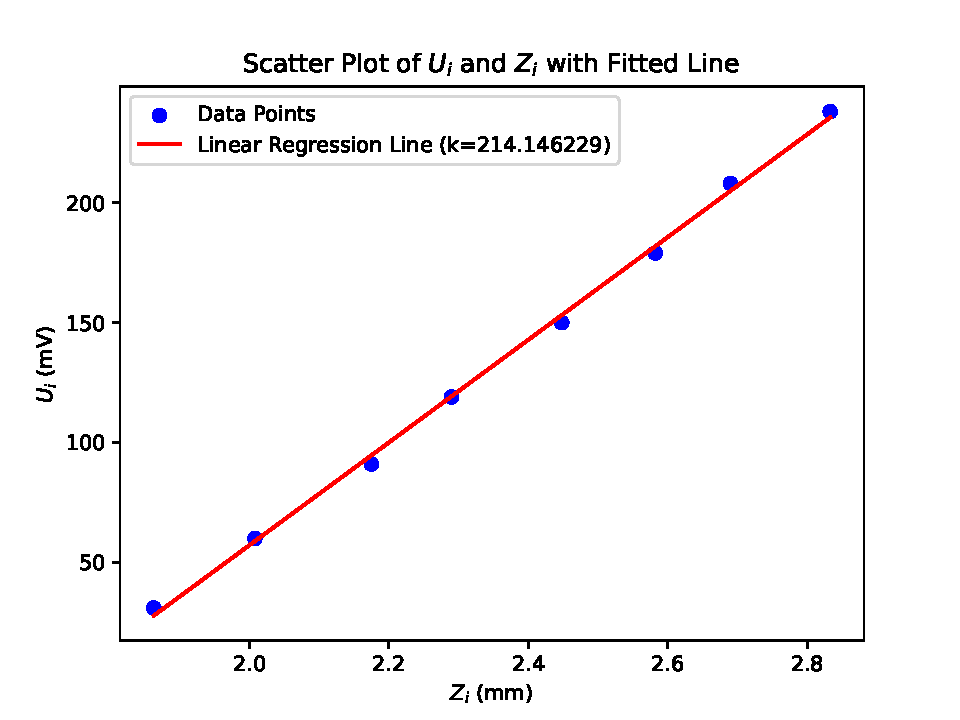
\includegraphics[width=0.6\textwidth]{./linear_regression_of_ui_and_zi.pdf}  % 将 "example-image" 替换为图片的文件名
\end{figure}

由图可知霍尔传感器的灵敏度为

\[k = 214.7 \, \text{mV} \cdot \text{mm}^{-1}\]

\subsection{总结与思考}

\subsubsection{实验过程中需要注意的问题}

\begin{enumerate}
  \item 在实验过程中需要注意，转动悬臂调整拉力时必须保证实验起始的时候是样品刚刚受到拉力开始弯曲的位置。不能在还没开始受到拉力的位置就开始测量，否则实验过程中霍尔电压将先往反方向变化，造成实验结果有较大的误差。
  \item 在实验过程中，需要特别注意不能将悬臂往反方向调，因此在转动悬臂的过程中要特别小心，避免超出读数范围。
  \item 读显微镜示数时要严格参照规则，不要受到直觉的影响，以免读数不准确。
\end{enumerate}

\subsubsection{思考题}

\begin{enumerate}
    \item 弯曲法测杨氏模量实验，主要测量误差有哪些？请估算各因素的不确定度。
    \begin{itemize}
        \item 主要测量误差包括：
        \begin{enumerate}
            \item \textbf{长度测量误差}：不确定度约为 $\pm 0.13 \, \text{mm}$。
            \item \textbf{宽度测量误差}：不确定度约为 $\pm 0.02 \, \text{mm}$。
            \item \textbf{厚度测量误差}：不确定度约为 $\pm 0.002 \, \text{mm}$。
            \item \textbf{弯曲位移测量误差}：不确定度约为 $\pm 0.01 \, \text{mm}$。
        \end{enumerate}
        \item 综合不确定度可通过误差传递公式计算，取各测量误差的平方和的平方根作为总不确定度。
    \end{itemize}
    
    \item 用霍尔位置传感器法测位移有什么优点？
    \begin{itemize}
        \item 霍尔位置传感器法测位移的优点包括：
        \begin{enumerate}
            \item \textbf{高灵敏度}：霍尔传感器能检测微小的位移变化，适合高精度的位移测量。
            \item \textbf{非接触测量}：通过磁场检测位移，无需接触被测物体，减少机械磨损和系统干扰。
            \item \textbf{良好的线性度}：霍尔传感器在一定范围内具有较好的线性度，便于精确测量和数据处理。
            \item \textbf{响应速度快}：适用于动态位移测量，不易受外界振动的影响。
        \end{enumerate}
    \end{itemize}
\end{enumerate}





\section{动态法测量杨氏模量}

\subsection{实验用具}

\begin{table}[h!]
\centering
\caption{实验用具清单}
\begin{tabular}{|l|l|}
\hline
\textbf{设备名称} & \textbf{型号或说明} \\ \hline
动态杨氏模量测试台 & DHY-2A 型 \\ \hline
振动力学通用信号源 & DH0803 \\ \hline
通用示波器 & - \\ \hline
测试棒 & 铜、不锈钢 \\ \hline
悬线 & - \\ \hline
专用连接导线 & - \\ \hline
天平 & - \\ \hline
游标卡尺 & - \\ \hline
螺旋测微计 & - \\ \hline
\end{tabular}
\end{table}

\subsection{实验原理}

\subsubsection*{横振动方程}
棒的横振动方程表示为：

\[
\frac{\partial^4 y}{\partial x^4} + \frac{-\rho S \frac{\partial^2 y}{\partial t^2}}{YJ} = 0
\]

其中 \(y\) 为振动位移，\(Y\) 为杨氏模量，\(S\) 为横截面积，\(J\) 为转动惯量，\(\rho\) 为密度，\(x\) 为位置坐标，\(t\) 为时间。

采用分离变量法，令 \(y(x, t) = X(x)T(t)\)，得：

\[
\frac{1}{X} \frac{d^4 X}{dx^4} = -\frac{\rho S}{YJ} \frac{1}{T} \frac{d^2 T}{dt^2} = K_4^4
\]

其中 \(K_4\) 为分离常数。两方程的解为：

\[
\frac{d^4 X}{dx^4} - K_4^4 X = 0, \quad \frac{d^2 T}{dt^2} + \frac{K_4^4 YJ}{\rho S} T = 0
\]

由此得通解：

\[
y(x, t) = (A_1 \cosh K_x + A_2 \sinh K_x + B_1 \cos K_x + B_2 \sin K_x) \cos (\omega t + \varphi)
\]

其中频率 \(\omega = \left( \frac{K_4^4 YJ}{\rho S} \right)^{1/2}\)。\(A_1, A_2, B_1, B_2, \varphi\) 为待定系数。

\subsubsection*{边界条件与超越方程}

对于长度 \(L\)、两端自由的棒，其边界条件为自由端横向力与弯矩为零，即：

\[
\left. \frac{d^3 X}{dx^3} \right|_{x=0, L} = 0, \quad \left. \frac{d^2 X}{dx^2} \right|_{x=0, L} = 0
\]

代入通解，得超越方程：

\[
\cos KL \cdot \cosh KL = 1
\]

数值求解的根依次为：\(K_n L = 0, 4.7300, 7.8532, 10.9956, \dots\)，趋近于 \((n - 1/2) \pi\)。

基频（或固有频率）对应 \(K_1 L = 4.7300\)。对于直径 \(d\)、长度 \(L\)、质量 \(m\) 的圆形棒，其基频 \(f_1\) 下的杨氏模量 \(Y\) 为：

\[
Y = 1.6067 \frac{L^3 m f_1^2}{d^4}
\]

测试棒在基频振动时有两个节点，理论上悬挂点应位于节点处以降低振动影响，可在节点旁取对称悬挂位置，外推求共振频率。

\subsubsection*{固有频率与共振频率关系}

固有频率 \(f_\text{固}\) 和共振频率 \(f_\text{共}\) 的关系为：

\[
f_\text{固} = f_\text{共} \sqrt{1 + \frac{1}{4Q^2}}
\]

其中 \(Q\) 为机械品质因素。通常 \(Q \approx 50\)，则两者差异约为 0.005\%，实验中可用共振频率近似代替固有频率。

\subsection{实验内容}


\begin{enumerate}
    \item \textbf{测量测试棒参数} \\
    测量测试棒的长度 \(L\)、直径 \(d\)、质量 \(m\)。为提高精度，每项测量重复3至5次。
    
    \item \textbf{测量共振频率 \(f_1\)}
    \begin{enumerate}
        \item \textbf{安装测试棒} \\
        将测试棒水平悬挂在两悬线上，悬线垂直于棒的轴向，挂点距离棒端点分别为 \(0.0365L\) 和 \(0.9635L\)。
        
        \item \textbf{连接设备} \\
        按实验要求连接测试台、信号源和示波器。
        
        \item \textbf{开机} \\
        打开示波器和信号源，调整示波器进入正常工作状态。
        
        \item \textbf{鉴频与测量} \\
        待测试棒稳定后，调节信号源频率和幅度，寻找共振频率 \(f_1\)。当示波器显示振幅极大值时，微调频率至最大振幅处。利用阻尼法验证基频共振：轻触测试棒不同位置，确认出现两个波节即为基频。记录共振频率 \(f_1\)。
        
        \item \textbf{多点测量} \\
        重复测量并记录棒的共振频率 \(f_1\)，悬线挂点位置依次为：\(0.099L\) 和 \(0.901L\)、\(0.1615L\) 和 \(0.8385L\)、\(0.224L\) 和 \(0.776L\)、\(0.2865L\) 和 \(0.7135L\)、\(0.349L\) 和 \(0.651L\)、\(0.415L\) 和 \(0.585L\)，记录结果。
        
        \item \textbf{注意事项} \\
        由于设备限制，部分设备在位置 \(0.0365L\) 和 \(0.9635L\) 处无法使悬线竖直，需跳过该点的测量。
    \end{enumerate}
\end{enumerate}

\subsection{数据整理与计算}

通过对铸铁棒的测量，知道其长度 \(L = 180.0\) mm，直径 \(d = 5.998\) mm，质量 \(m = 39.81\) g。铸铁棒悬挂点位置和共振频率的关系如下表所示：

\begin{table}[h]
    \centering
    \begin{tabular}{|c|c|c|c|c|c|c|c|c|}
        \hline
        序号 & 1 & 2 & 3 & 4 & 5 & 6 & 7 & 8 \\ \hline
        悬挂点位置 \( x \)/mm & 20 & 25 & 30 & 35 & 45 & 50 & 55 & 60 \\ \hline
        \( x/L \) & 0.111 & 0.138 & 0.167 & 0.194 & 0.250 & 0.278 & 0.306 & 0.333 \\ \hline
        共振频率 \( f_1 \)/Hz & 827.100 & 826.812 & 826.522 & 826.362 & 826.492 & 826.582 & 826.682 & 827.172 \\ \hline
    \end{tabular}
    \caption{悬挂点位置和共振频率关系}
\end{table}

\begin{figure}[H]
    \centering
    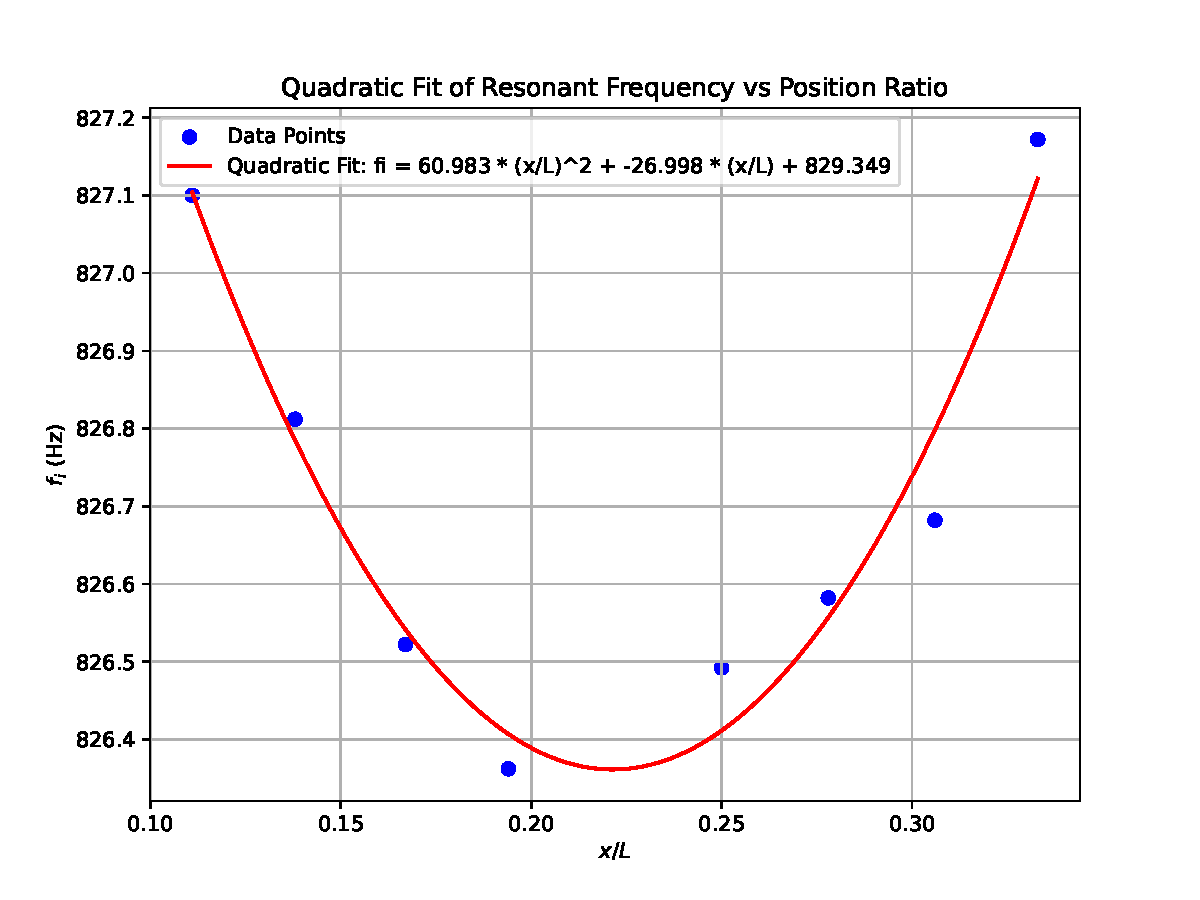
\includegraphics[width=0.6\textwidth]{./quadratic_fit_of_fi_and_x.pdf}  % 将 "example-image" 替换为图片的文件名
\end{figure}

由图可知，$f_1$关于$\frac{x}{L}$的拟合方程为

\[ f_1 = 60.983 \left( \frac{x}{L} \right)^2 - 26.998 \left( \frac{x}{L} \right) + 829.349 \]

知道当$\frac{x}{L} = 0.22136$时，$f_1 = 826.36$Hz

\subsubsection{铸铁杨氏模量的计算}

根据公式$Y = 1.6067 \frac{L^3 m f_1^2}{d^4}$，铸铁杨氏模量的计算结果如下

\[ Y = 1.6067 \frac{180.0^3 \times 39.81 \times 826.36^2}{(5.998)^4} = 1.97 \times 10^{11} \, \text{N} \cdot \text{m}^{-2} \]

我们知道铸铁杨氏模量的标准数据为$1.52 \times 10^{11}$N·m$^{-2}$，我们可以计算相对误差

\[ E_r (Y) = \frac{|Y - Y_0|}{Y_0} \times 100\% = \frac{(1.97 - 1.52)}{1.52} \times 100\% = 29.6\% \]

\subsection{总结与思考}

\subsubsection{实验过程中需要注意的问题}

在不知道共振频率的情况下，我们可能会将频率调得非常大，此时金属棒也将出现类似共振的波形。但此时的频率并不是共振的基频。此时我们可以通过阻尼法验证基频共振：轻触测试棒不同位置，确认出现两个波节即为基频。在测量过程中，我们也需要注意悬挂线要与棒垂直，以减小误差。同时，判断是否达到共振一定要读取示波器上的幅值数据，而不是单纯地通过眼睛判断。

\subsubsection{思考题}

\begin{enumerate}
    \item 外延测量法有什么特点？使用时应注意什么问题？（外推法还将在“实验五.气垫导轨实验”中见到）
    \begin{itemize}
        \item 外延测量法的特点：
        \begin{enumerate}
            \item \textbf{适用于不容易直接测量的量}：外延测量法通过间接推算得到测量值，常用于无法直接测量的物理量，例如在本实验中直接测量40mm处的数值时会发现没有明显的波形，此时就需要借助外延法。
            \item \textbf{简便且快速}：通过合理的模型和数据推算，可以较为迅速地得到需要的结果，避免直接测量的复杂性。
            \item \textbf{依赖于准确的理论模型}：外延测量法的准确性高度依赖于所采用的模型和假设的准确性，例如是选择线性拟合还是抛物线拟合。
        \end{enumerate}
        \item 使用时应注意的问题：
        \begin{enumerate}
            \item \textbf{理论模型的可靠性}：所使用的模型应与实际情况相符，否则推算出的结果可能出现较大误差。
            \item \textbf{实验数据的准确性}：外延法常需要较多的实验数据，数据误差会传递并影响最终结果的准确性。
            \item \textbf{外推范围的合理性}：外延法常用于推算超出已知范围的量，外推的范围应尽量接近实验数据的实际范围，以避免过大的误差。
        \end{enumerate}
    \end{itemize}
    
    \item 物体的固有频率和共振频率有什么不同？它们之间有何关系？
    \begin{itemize}
        \item \textbf{固有频率}是指物体在没有外界激励的情况下，因其形状、尺寸、材质等固有特性而自然振动的频率。每个物体都有其特定的固有频率。
        \item \textbf{共振频率}是指当外部周期性力的频率与物体的固有频率相匹配时，物体会发生共振现象，即振动幅度急剧增大，产生强烈的响应。
        \item \textbf{关系}：固有频率和共振频率的关系可以用以下公式来表述\[f_\text{固} = f_\text{共} \sqrt{1 + \frac{1}{4Q^2}}\]其中 \(Q\) 为机械品质因素。通常 \(Q \approx 50\)，则两者差异约为 0.005\%，由于这个差异非常小，因此在本实验中用共振频率近似代替固有频率。
    \end{itemize}
\end{enumerate}

\end{document}

% VScode 常用快捷键：

% F2:                       变量重命名
% Ctrl + Enter:             行中换行
% Alt + up/down:            上下移行
% 鼠标中键 + 移动:           快速多光标
% Shift + Alt + up/down:    上下复制
% Ctrl + left/right:        左右跳单词
% Ctrl + Backspace/Delete:  左右删单词    
% Shift + Delete:           删除此行
% Ctrl + J:                 打开 VScode 下栏(输出栏)
% Ctrl + B:                 打开 VScode 左栏(目录栏)
% Ctrl + `:                 打开 VScode 终端栏
% Ctrl + 0:                 定位文件
% Ctrl + Tab:               切换已打开的文件(切标签)
% Ctrl + Shift + P:         打开全局命令(设置)

% Latex 常用快捷键：

% Ctrl + Alt + J:           由代码定位到PDF


